\chapter{Introduction}
This report and the corresponding documentation with its appendix is written as the documentation of the development process of the AU2 car, the dynamo-meter dubbed Rolling Road and the GUI developed for use with the Rolling Road. The products being developed are made to either compete in the Shell Eco Marathon or work as test benches for the car competing. The development process is accomplished in colaboration with Aarhus School of Engineering (ASE) as the 4\textsuperscript{th} term project. This means that the report covers three major systems:

\begin{itemize}
	\item{AU2}
	\item{Rolling Road}
	\item{GUI}
\end{itemize}

AU2 is the car built to compete in the Shell Eco-Marathon. In this report the electrical and embedded systems developed for controlling the car will be described. 

The Rolling Road and GUI are coherent systems, although they can function independently. This report will cover the electrical system, embedded- and desktop-software for Rolling Road and the GUI. 

This report will only scratch the surface. For in-depth design and implementation features, the rader is referred to the associated documentation. These documentations includes all calculations and many of the design choices made as well.  

The products being developed will serve as a working product that has been thoroughly tested. This is done so that no breakdown occurs during the race. It will also serve as a guideline for future work, for other students who will be working on future iterations of AU2. It is therefore important that the documentation provided alongside this report must be as comprehensive as possible.

Throughout the work with developing this car, there have been many hours of collaboration with a team of mechanical engineers who are responsible for designing and building the vehicle's body. The interdisciplinary work with the mechanical engineers have made this a rather large project and therefore required cross-group project-management; which was absent for large parts of the project. 

The report and all of the documentation has been written in English to keep it coherent with previous documentations developed for Shell Eco Marathon. Furthermore, the technical documentation which was required to be delivered to Shell for the technical inspection of the car, must be in english and therefore it was easier and more convenient to be able to copy/paste from this report and the associated documents.

\section{List of terms}
The following list explains the various terms which are used in this report to refer to various relevant items from all three systems:
\begin{itemize}
	\item \textbf{AU2}\\
	AU2 is the newest car made to compete in SEM 2016. When AU2 is herein referred, it is the entire electrical system and the embedded software. 
	\item \textbf{SEM}\\
	The Shell Eco-Marathon 2016 which is held at London and which one of the goals of this project has been to compete in.
	\item \textbf{AU - Shell Eco-Marathon Team}\\
	The complete team consisting of both electrical and mechanical engineers who developing AU2 in order to compete in Shell Eco-Marathon.
	\item \textbf{PSoC}\\
	Refers to the CY8CKIT-059 PSoC 5LP Prototype Kit which is used to build the Control Unit in Rolling Road and the Motor Controller in AU2.
	\item \textbf{BMS}\\
	The BMS refers to the battery management system used for monitoring the batteries. 
	\item \textbf{MCS}\\
	When the abbreviation MCS is used, it refers to the PCB developed to contain the motor controller amongst other things.
	\item \textbf{Zenith33}\\
	A electrically propulsed car which had been designed to compete in Shell Eco-Marathon 2014\cite{BAC_zenith33} on behalf of AU. Due to its design, this car was not allowed to compete in SEM 2016. However, due to the mechanical body of AU2 being developed in parallel many of the tests were performed using Zenith33.
	\item \textbf{Previous dynamometer}\\
	An earlier version of Rolling Road called 'Teststand tilBørsteløs DC Motor'\cite{BAC_rullefelt}. 
\end{itemize}

\section{Reading guide}
This report gives the reader an insight into the different aspects of the project-development; such as the key documentation to gain an overview of the system and some of the challenges met while developing. The report can be split into multiple parts:

\textbf{First part} of the report gives a quick overview of the system and the team-members who helped develop the system. It includes chapter 1 through 4.

\textbf{Second part} describes the process used to manage the project and programs used to in the development process, and includes chapter 5 and 6.

\textbf{Third part} describes the requirements, overall architecture and the design considerations, implementation and test of different systems developed as a part of this project. This part includes chapter 7 through 10.

\textbf{Fourth part} includes chapter 11 and 12. It talks about the results and what could be done in the future to enhance the product. Lastly, it includes some of the experience gained both as a group and individually for each team member.

\textbf{Fifth part} concludes the project as a whole and consists of chapter 14.

\clearpage
\section{Areas of responsibility}
In the following table the team members will describe their primary responsibilities during the project. 

\begin{tabular}[c]{|p{3cm}| p{5cm} | p{6cm}|}
	\hline
	\textbf{Member} & \textbf{Area of responsibility} & \textbf{Description}\\\hline
	
	% Jens
	\phantom{Test}
	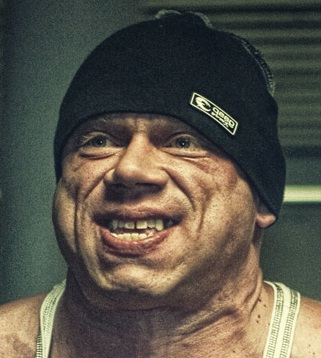
\includegraphics[width=3cm]{Introduction/TeamPictures/Jens} & \multirow{2}{5cm}{Project leader and communication coordinator.\newline \newline Hardware and software developer on AU2's Battery Management System.\newline \newline System architecture for Battery Management System.} & \multirow{2}{6cm}{As the project leader I have fx been responsible for communicating with the mechanical engineering team.\newline \newline I've also been responsible for the system description and system architecture of the Battery Management System, while also be responsible for the design and implementation of it.} \\
	Jens Peter M.\newline Nymann & & \\ \hline
	
	%Jonas
	\phantom{Test}
	
\includegraphics[width=3cm]{Introduction/TeamPictures/Jonas} & \multirow{2}{5cm}{SCRUM-Master and software developer on the Rolling Road GUI and AU2} & \multirow{2}{6cm}{As the SCRUM-master i've been in charge of the bi-weekly SCRUM standup meetings and planning of new sprints.\\
		I was also in charge of the Rolling Road GUI Application and in addition wrote the SD-Card logging software for the AU2.
		} \\
	Jonas M. Hansen & & \\ \hline
	
	%Jonathan
	\phantom{Test}
	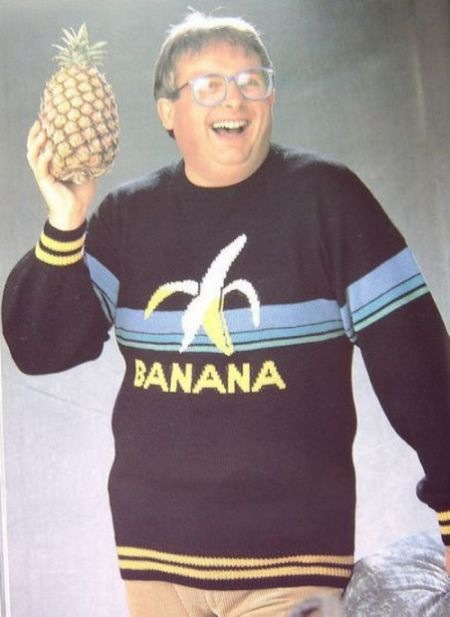
\includegraphics[width=3cm]{Introduction/TeamPictures/Jonathan} & \multirow{2}{5cm}{Area of responsibility goes here} & \multirow{2}{6cm}{Description goes here plzzzzzzzzzzzzzzzz} \\
	Jonathan Schougaard & & \\ \hline
\end{tabular}

\newpage
\begin{tabular}[c]{|p{3cm}| p{5cm} | p{6cm}|}
	\hline
	\textbf{Member} & \textbf{Area of responsibility} & \textbf{Description}\\\hline
	
	%Laimonas
	\phantom{Test}
	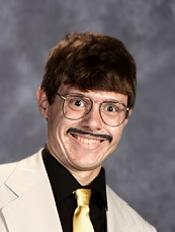
\includegraphics[width=3cm]{Introduction/TeamPictures/Laimonas} & \multirow{2}{5cm}{Hardware and software development on AU2's Battery Management System} & \multirow{2}{6cm}{I have primarily been responsible for the Battery Management System. This includes assignments such as reverse engineering, design and implementation as well as software and hardware optimization on the BMS.} \\
	Laimonas I. \newline Bendikas & & \\ \hline
		
	%Thomas R
	\phantom{Test}
	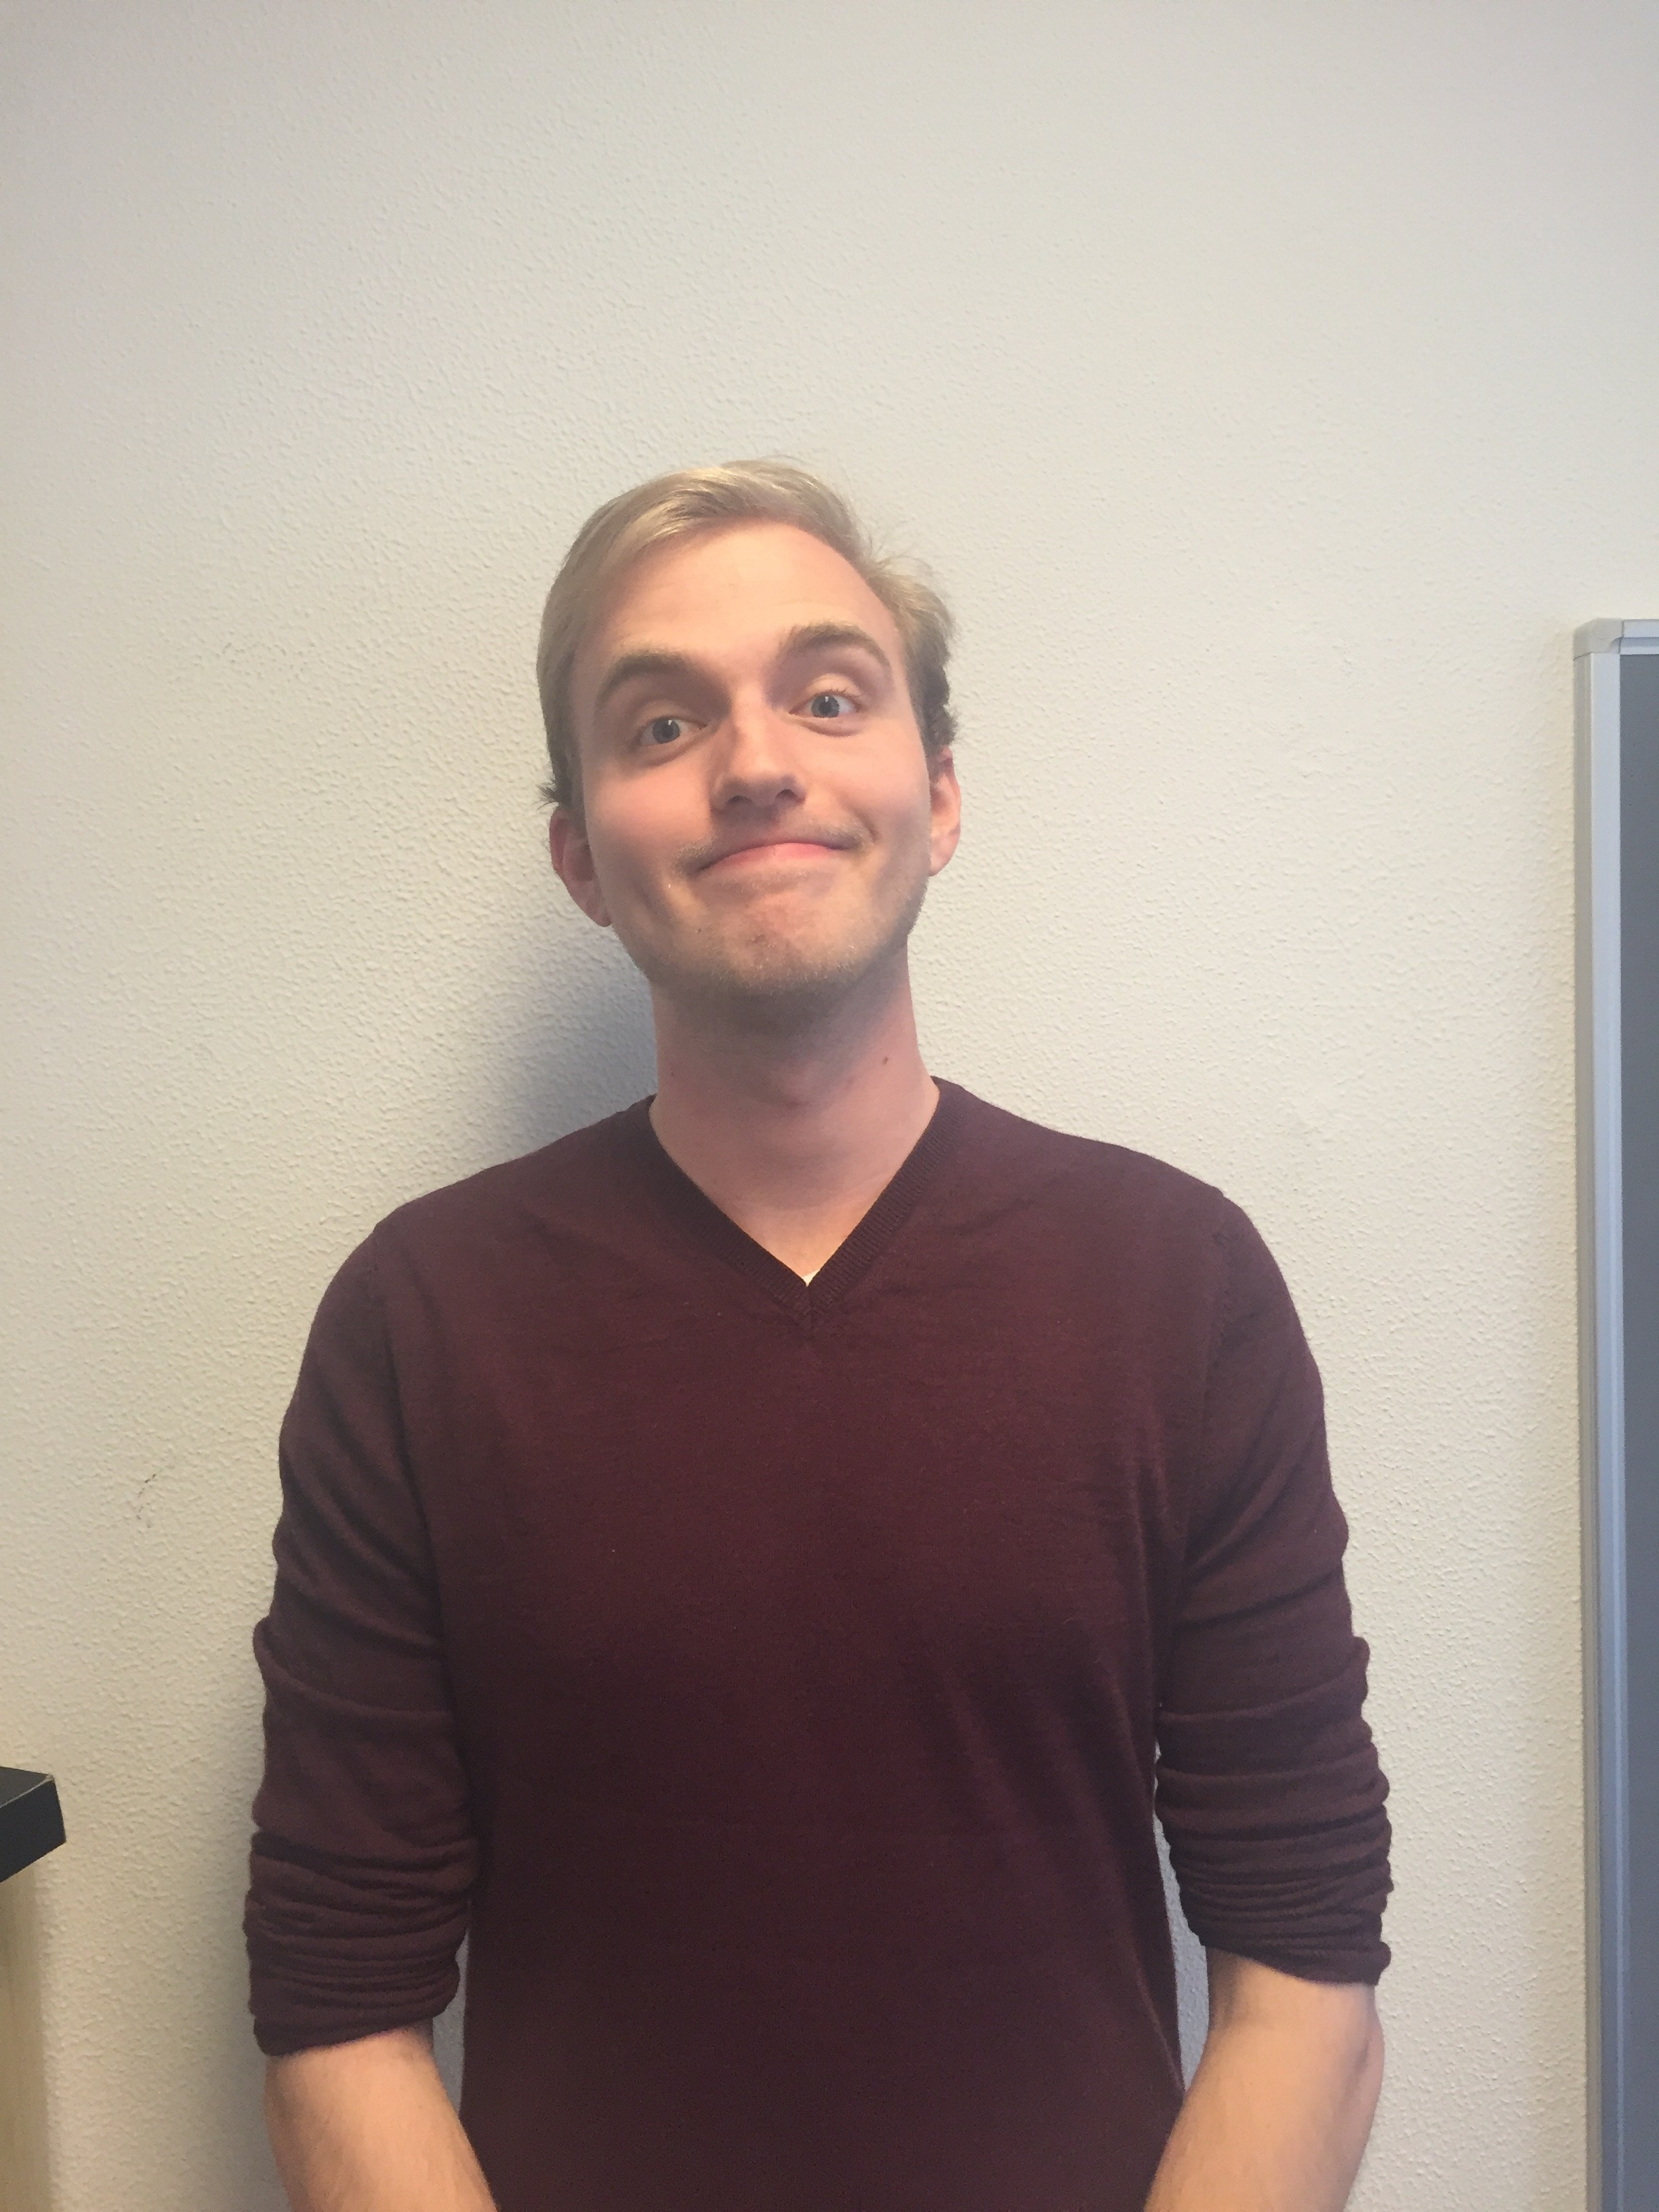
\includegraphics[width=3cm]{Introduction/TeamPictures/ThomasR} & \multirow{2}{5cm}{Hardware analysis, design and implementation on Rolling Road.} & \multirow{2}{6cm}{I've been responsible for for analysing the previous dynamometer-system in order to create the hardware in Rolling Road.} \\
	Thomas S. \newline Rasmussen & & \\ \hline
		
	%Thomas N
	\phantom{Test}                                                                                                                                                                                                                                                      
	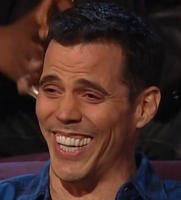
\includegraphics[width=3cm]{Introduction/TeamPictures/ThomasN} & \multirow{2}{5cm}{Hardware development for AU2 \newline \newline Protocol development for RR} & \multirow{2}{6cm}{I have been responsible for the design and implementation of the hardware for AU2. Furthermore I have developed the Protocol for Rolling Road} \\
	Thomas B. \newline Nielsen & & \\ \hline
\end{tabular}